%----------------------------------------------------------------------
% demonstration on how to include graphics into an article
\documentclass[a4paper,11pt]{article}
\usepackage{graphicx}                  % This is needed for including figures and graphics
\DeclareGraphicsRule{.tif}{png}{.png}{`convert #1 `dirname #1`/`basename #1 .tif`.png}

%----------------------------------------------------------------------
\begin{document}
\author{Christian Monstein, Institute of Astronomy, Z\"{u}rich, Switzerland}
\title{Callisto solar radio spectrometer}
\maketitle
%----------------------------------------------------------------------
\abstract{This document demonstrates on how to include plots from
Python.}
%----------------------------------------------------------------------
\section{Introduction}
Python is an easy and cheap too to generate plots.
%----------------------------------------------------------------------
\begin{figure} % overview total
\centering
   %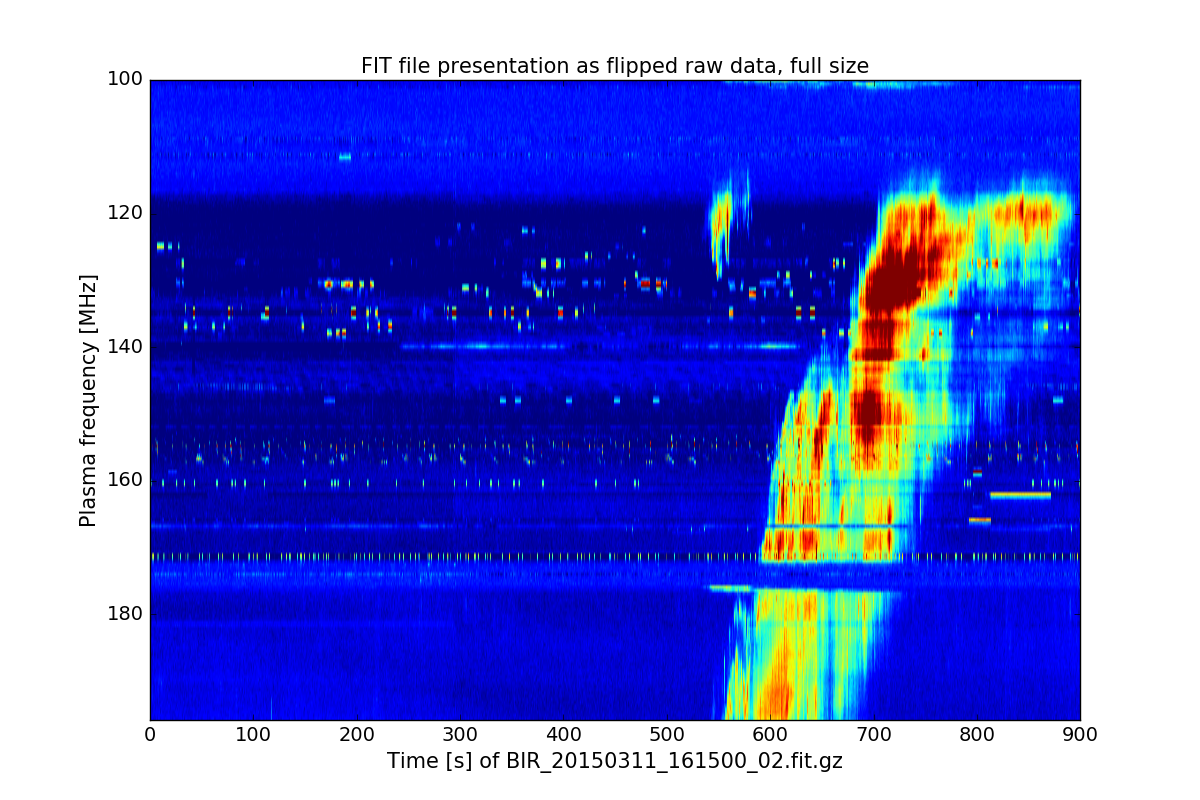
\includegraphics[natwidth=1200bp,natheight=800bp, width=\textwidth]{2D_flipud.png} % or
   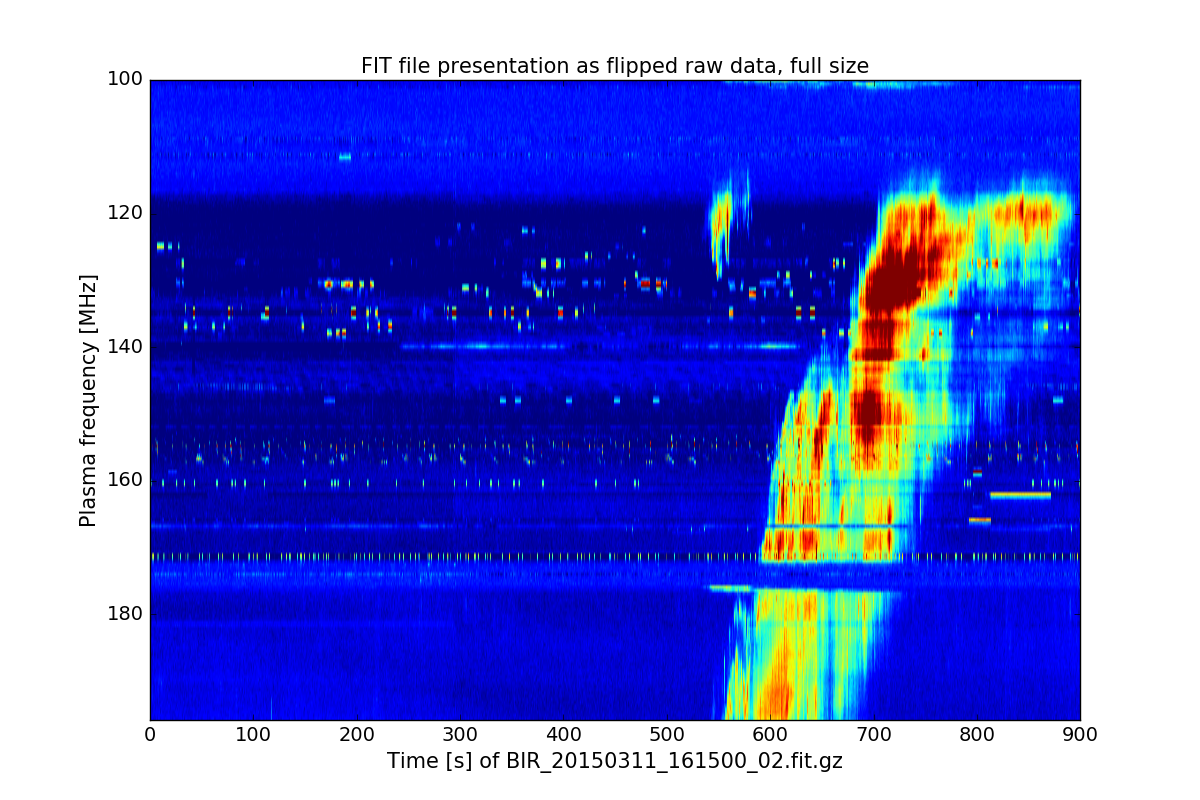
\includegraphics[natwidth=1200bp,natheight=800bp, scale=0.5]{2D_flipud.png}%0.42
\caption{1st light from Bir, a type II burst.\label{1stlight}}
\end{figure}
%----------------------------------------------------------------------
\section{Conclusions}
The Callisto instrument proved to be a cheap but powerful tool for
spectroscopy.
%----------------------------------------------------------------------
\end{document}
